\chapter{Epidemiología del cáncer}

La Epidemiología se ha definido tradicionalmente como la ciencia que estudia la distribución y los determinantes de la enfermedad en los seres humanos \cite{MacMahon1970}. En una definición más moderna, no limitada exclusivamente a la enfermedad, la Epidemiología se define como el estudio de la aparición y distribución de los estados o acontecimientos relacionados con la salud en poblaciones específicas, incluyendo el estudio de los determinantes de estos estados, y la aplicación de este conocimiento al control de los problemas de la salud \cite{Porta2008}.

\section{Indicadores epidemiológicos}

Para medir en la población el impacto del cáncer se utilizan principalmente cuatro indicadores:

\begin{itemize}
	\item \textbf{Incidencia} (casos nuevos). Mide el riesgo de presentar cáncer.
	\item \textbf{Mortalidad} (defunciones). Mide el riesgo de morir por cáncer.
	\item \textbf{Supervivencia} (porcentaje de casos vivos). Mide la historia natural del cáncer y efectividad del tratamiento.
	\item \textbf{Prevalencia} (casos nuevos y antiguos, vivos). Mide la carga asistencial de la enfermedad.
\end{itemize}

Además, se puede examinar la evolución de cada indicador a lo largo del tiempo, hablando así de tendencias de la incidencia, de la mortalidad, de la supervivencia o de la prevalencia.\\

\textcolor{blue}{(Ver si se incluyen tendencias, sería conveniente al menos para incidencia y/o mortalidad)}

% ---------------------------------

\subsection{Fuentes de información}

A nivel mundial, las estadísticas de cáncer las proporciona el \textit{Global Cancer Observatory} (GCO), una plataforma web de la \textit{International Agency for Research on Cancer}, de la Organización Mundial de la Salud \cite{Bray2018, GCO}.\\

El organismo equivalente al GCO a nivel europeo es el \textit{European Cancer Information System} (ECIS), de reciente creación y apoyado por la Comisión Europea \cite{ECIS, ECIS2}.\\

Aunque estos organismos proporcionan estadísticas sobre cáncer en España, también existen fuentes a nivel nacional que cuentan con datos más actualizados y con distinta metodología. La Red Española de Registros de Cáncer (REDECAN) publica periódicamente datos sobre incidencia y supervivencia de cáncer en España \cite{REDECAN2020, Guevara2019}, mientras que las estadísticas de mortalidad por cáncer se pueden calcular a partir de las defunciones que publica el Ministerio de Sanidad, Consumo y Bienestar Social del Gobierno de España \cite{MSCBS} y la población que proporciona el Instituto Nacional de Estadística \cite{INEpob}.\\

\textcolor{red}{SUPERVIVENCIA: CONCORD y/o EUROCARE}.


\section{Incidencia de cáncer}

\subsection{Metodología}

Para medir de manera precisa la incidencia de cáncer en una población es necesaria la existencia de un Registro de Cáncer Poblacional. Estas entidades se dedican a registrar exhaustivamente todos los casos de cáncer diagnosticados en un área geográfica, y sus datos son muy útiles para todo tipo de estudios epidemiológicos. Algunos de estos Registros cubren la población de todo un país (por ejemplo, Canadá) mientras que otros cubren regiones concretas (por ejemplo, la provincia de Granada). Desgraciadamente, muchas áreas geográficas no están cubiertas por un Registro de Cáncer Poblacional. Es el caso de España, en el que sólo el 27\% de la población está cubierta por un Registro de Cáncer Poblacional \cite{Redondo-Sanchez2019}. Para conocer de manera estimada la incidencia de cáncer en territorios sin Registro de Cáncer Poblacional o proyectar la incidencia a años posteriores se utilizan diversos métodos matemáticos y estadísticos \cite{Bray2018, GCO, ECIS, ECIS2, REDECAN2020, Redondo-Sanchez2019}.\\

Con respecto a las medidas usadas para reportar la incidencia, la más sencilla y fácil de interpretar es el número nuevo de casos de cáncer, enmarcado siempre en un periodo concreto de tiempo y un área geográfica. A partir del número de casos se puede calcular la tasa bruta (TB), un indicador que tiene en cuenta el tamaño de la población y que se suele calcular por 100.000 habitantes \cite{IARC1995}.\\

$$\text{TB}  = 100.000 \cdot \dfrac{\text{Número de casos nuevos}}{\text{Personas-año a riesgo}}$$\\

Para permitir comparaciones entre distintas poblaciones, o la misma población en momentos distintos, es necesario tener en cuenta la estructura de edad de la población. Para responder a esta motivación se define la tasa estandarizada por edad (ASR por sus siglas en inglés, \textit{Age-Standardised Rate}) como aquella tasa que habría en la población de estudio si tuviese exactamente la misma estructura de edad que una población estándar predefinida \cite{IARC1995}. La definición de la tasa estandarizada por edad para 18 grupos de edad quinquenales (0-4 años, 5-9 años, $\dots$, 80-84 años, 85 años y más) es la siguiente:

$$\text{ASR} = \sum_{i = 1}^{18} \omega_i \dfrac{N_i}{P_i} $$
donde $N_i$ y $P_i$ son respectivamente el número de casos incidentes y la población en el $i$-ésimo grupo de edad, y $\omega_i$ es el peso que toma la población de referencia en el grupo $i$-ésimo, con $\sum_{i = 1}^{18}\omega_i = 100.000$. Los valores de ${\omega_i}$ están predefinidos en base a poblaciones estándar, siendo las más utilizadas en nuestro contexto las siguientes:

\begin{itemize}
	
	\item Población mundial. Propuesta por primera vez en 1960 \cite{SegiM.1960} y modificada más tarde en 1966 \cite{Doll1966}, permite realizar comparaciones a nivel mundial.
		
	\item Antigua población estándar europea. Propuesta en 1976 \cite{Waterhouse1976} basándose en la estructura de edad de varias poblaciones escandinavas, permite comparaciones entre zonas europeas.
	
	\item Nueva población estándar europea. En el año 2013, la Oficina Europea de Estadística (EUROSTAT) realiza una revisión de la población estándar europea con el objetivo de que la población refleje fielmente el envejecimiento existente en la población europea \cite{EUROSTAT2013}. Debido a su novedad, el uso de esta población aún no está ampliamente extendido en los organismos internacionales \cite{ECIS2} y en ocasiones se reportan las dos tasas estandarizadas por las poblaciones estándar antigua y nueva \cite{ECIS}.
	

\end{itemize}

En la Tabla 1 se muestran los pesos para cada una de las poblaciones de referencia mencionadas anteriormente.\\

\newpage
\textbf{Tabla 1}. Pesos de las poblaciones estándar para el cálculo de tasas estandarizadas por edad.
\begin{table}[H]
	\begin{tabular}{|r|r|r|r|}
		\hline		
		Grupo de edad  &  \begin{tabular}[r]{@{}r@{}}Población estándar\\ mundial\end{tabular}  &  \begin{tabular}[r]{@{}r@{}}Población estándar\\ europea 1976\end{tabular}  &  \begin{tabular}[r]{@{}r@{}}Población estándar\\ europea 2013\end{tabular}\\\hline
		
		0-4 años  &  12.000  &  8.000  &  5.000\\
		5-9 años  &  10.000  &  7.000  &  5.500\\
		10-14 años  &  9.000  &  7.000  &  5.500\\
		15-19 años  &  9.000  &  7.000  &  5.500\\
		20-24 años  &  8.000  &  7.000  &  6.000\\
		25-29 años  &  8.000  &  7.000  &  6.000\\
		30-34 años  &  6.000  &  7.000  &  6.500\\
		35-39 años  &  6.000  &  7.000  &  7.000\\
		40-44 años  &  6.000  &  7.000  &  7.000\\
		45-49 años  &  6.000  &  7.000  &  7.000\\
		50-54 años  &  5.000  &  7.000  &  7.000\\
		55-59 años  &  4.000  &  6.000  &  6.500\\
		60-64 años  &  4.000  &  5.000  &  6.000\\
		65-69 años  &  3.000  &  4.000  &  5.500\\
		70-74 años  &  2.000  &  3.000  &  5.000\\
		75-79 años  &  1.000  &  2.000  &  4.000\\
		80-84 años  &  500  &  1.000  &  2.500\\
		$\geq$85 años  &  500  &  1.000  &  2.500\\\hline
	\end{tabular}
\end{table}

Para utilizar notación internacional, la tasa estandarizada por la población mundial se notará ASR-W (de \textit{World standard population}), la tasa estandarizada por la población europea de 1976 se notará ASR-oE (\textit{old European standard population}) y la de 2013 se notará ASR-nE (\textit{new European standard population}).\\


\subsection{Incidencia del total del cáncer excepto piel no melanoma}

El cáncer de piel no melanoma se suele excluir al reportar datos de incidencia del total del cáncer, debido a que es muy frecuente y cuenta con buen pronóstico, por lo que no se suele registrar en los Registros de Cáncer Poblacionales \cite{Gordon2013, Madan2010}.\\

\textbf{\textcolor{red}{Figura XX}}. Diagrama de Marimekko/mosaico con la incidencia estimada de cáncer excepto piel no melanoma en el mundo para el año 2018. Ocho localizaciones anatómicas más frecuentes en ambos sexos. Fuente: \textit{Global Cancer Observatory}, Organización Mundial de la Salud \cite{GCO}.
\begin{center}
	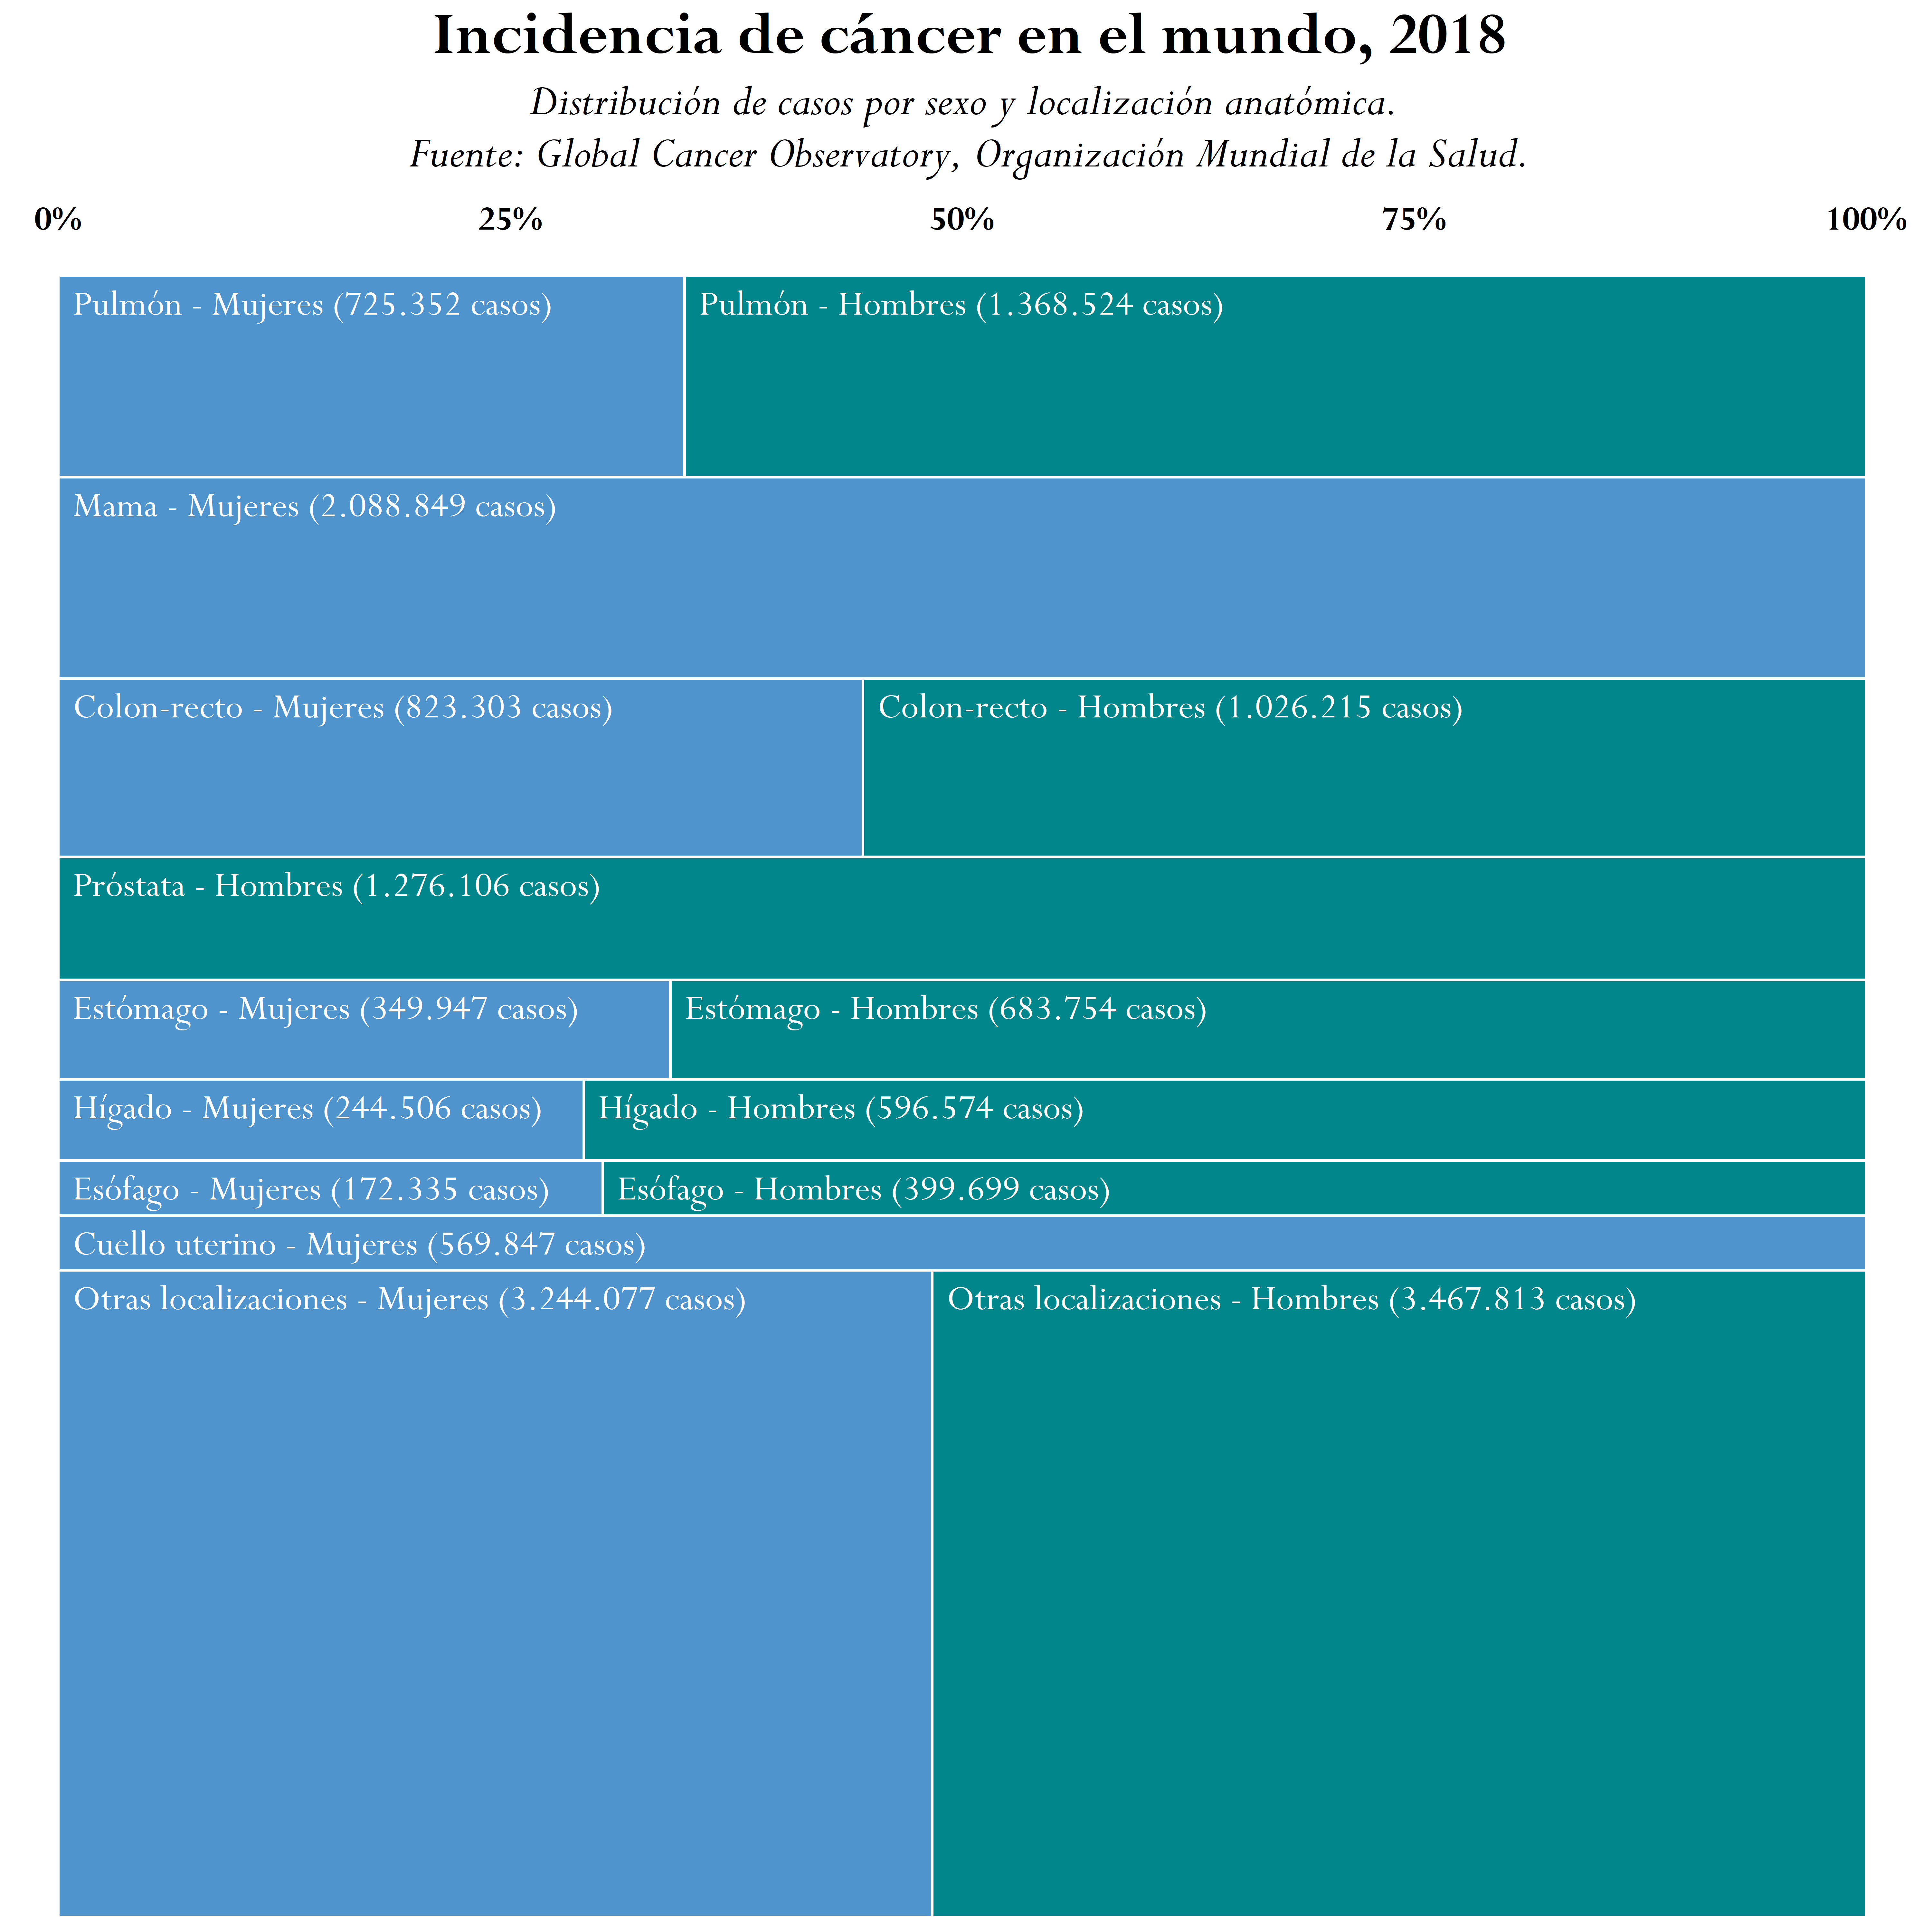
\includegraphics[width=1\textwidth]{figuras/marimekko_gco.png} \\
\end{center}


\newpage
\textbf{\textcolor{red}{Tabla X}}. Incidencia del total del cáncer excepto piel no melanoma en 2018, por sexo y población. Número de casos nuevos (N), tasa bruta (TB), tasa estandarizada por la población mundial (ASR-W),  tasa estandarizada por la antigua población europea (ASR-oE) y  tasa estandarizada por la nueva población europea (ASR-nE).

\begin{table}[H]
	\begin{tabular}{|c|l|c|r|r|r|r|r|}
		\hline		

\multicolumn{1}{|c|}{Sexo} & \multicolumn{1}{|c|}{Población} & Fuente & \multicolumn{1}{|c|}{N} & \multicolumn{1}{|c|}{TB} & \multicolumn{1}{|c|}{ASR-W} & \multicolumn{1}{|c|}{ASR-oE} & \multicolumn{1}{|c|}{ASR-nE}\\\hline

\multirow{3}{*}{Hombres} & Mundo & GCO \cite{GCO} & 8.818.685 & 229,0 & 204,7 &  & \\
& Europa & ECIS \cite{ECIS} & 2.059.673 & 572,9 & 302,7 & 436,0 & 651,7\\
& España & ECIS \cite{ECIS} & 142.353 & 625,6 & 309,7 & 444,7 & 658,6\\\hline
\multirow{3}{*}{Mujeres} & Mundo & GCO \cite{GCO} & 8.218.216 & 217,3 & 175,6 &  & \\
& Europa & ECIS \cite{ECIS} & 1.851.644 & 481,8 & 242,7 & 332,6 & 451,2\\
& España & ECIS \cite{ECIS} & 106.647 & 451,1 & 218,4 & 298,5 & 401,7\\\hline
\multirow{3}{*}{\begin{tabular}[c]{@{}c@{}}Ambos\\sexos\end{tabular}} & Mundo & GCO \cite{GCO} & 17.036.901 & 223,2 & 187,8 &  & \\
& Europa & ECIS \cite{ECIS} & 3.911.317 & 525,8 & 266,7 & 374,3 & 531,9\\
& España & ECIS \cite{ECIS} & 249.000 & 536,7 & 259,4 & 363,8 & 515,3\\\hline

	\end{tabular}
\end{table}

A nivel nacional, REDECAN ha publicado estimaciones de la incidencia en España más recientes a las mostradas en la \textcolor{red}{Tabla X}, correspondientes al año 2020, \cite{REDECAN2020}. En este análisis se estima el número de casos de cáncer excepto piel no melanoma en 277.394 casos (57.8\% en hombres), con una tasa bruta de 588,0 por 100.000 habitantes, y tasas estandarizadas de 280,3 (ASR-W), 399,4 (ASR-oE) y 579,8 (ASR-nE).

\subsection{Incidencia de cáncer de hígado}

\newpage
\textbf{\textcolor{red}{Tabla X}}. Incidencia de cáncer de hígado en 2018, por sexo y población. Número de casos nuevos (N), tasa bruta (TB), tasa estandarizada por la población mundial (ASR-W),  tasa estandarizada por la antigua población europea (ASR-oE) y  tasa estandarizada por la nueva población europea (ASR-nE).

\begin{table}[H]
	\begin{tabular}{|c|l|c|r|r|r|r|r|}
		\hline		
		
		\multicolumn{1}{|c|}{Sexo} & \multicolumn{1}{|c|}{Población} & Fuente & \multicolumn{1}{|c|}{N} & \multicolumn{1}{|c|}{TB} & \multicolumn{1}{|c|}{ASR-W} & \multicolumn{1}{|c|}{ASR-oE} & \multicolumn{1}{|c|}{ASR-nE}\\\hline
		
\multirow{3}{*}{Hombres} & Mundo & GCO \cite{GCO} & 596.574 & 15,5 & 13,9 &  & \\
& Europa & ECIS \cite{ECIS} & 55.825 & 15,5 & 8,0 & 11,7 & 17,7\\
& España & ECIS \cite{ECIS} & 4.976 & 21,9 & 10,9 & 15,7 & 22,5\\\hline
\multirow{3}{*}{Mujeres} & Mundo & GCO \cite{GCO} & 244.506 & 6,5 & 4,9 &  & \\
& Europa & ECIS \cite{ECIS} & 26.641 & 6,9 & 2,7 & 4,0 & 6,3\\
& España & ECIS \cite{ECIS} & 1.654 & 7,0 & 2,4 & 3,6 & 6,0\\\hline
\multirow{3}{*}{\begin{tabular}[c]{@{}c@{}}Ambos\\sexos\end{tabular}} & Mundo & GCO \cite{GCO} & 841.080 & 11,0 & 9,3 &  & \\
& Europa & ECIS \cite{ECIS} & 82.466 & 11,1 & 5,1 & 7,4 & 11,3\\
& España & ECIS \cite{ECIS} & 6.630 & 14,3 & 6,5 & 9,3 & 13,6\\\hline
		
	\end{tabular}
\end{table}

En las estimaciones publicadas por REDECAN para 2020 se estiman en España 6.595 casos de cáncer de hígado (75,4\% en hombres), con una tasa bruta de 14,0 y tasas estandarizadas de 6,5 (ASR-W), 9,4 (ASR-oE) y 13,9 (ASR-nE) \cite{REDECAN2020}.

\subsection{Incidencia de cáncer de colon-recto}

\textbf{\textcolor{red}{Tabla X}}. Incidencia de cáncer de colon-recto en 2018, por sexo y población. Número de casos nuevos (N), tasa bruta (TB), tasa estandarizada por la población mundial (ASR-W),  tasa estandarizada por la antigua población europea (ASR-oE) y  tasa estandarizada por la nueva población europea (ASR-nE).

\begin{table}[H]
	\begin{tabular}{|c|l|c|r|r|r|r|r|}
		\hline		
		
		\multicolumn{1}{|c|}{Sexo} & \multicolumn{1}{|c|}{Población} & Fuente & \multicolumn{1}{|c|}{N} & \multicolumn{1}{|c|}{TB} & \multicolumn{1}{|c|}{ASR-W} & \multicolumn{1}{|c|}{ASR-oE} & \multicolumn{1}{|c|}{ASR-nE}\\\hline
		
\multirow{3}{*}{Hombres} & Mundo & GCO \cite{GCO} & 1.026.215 & 26,6 & 23,6 &  & \\
& Europa & ECIS \cite{ECIS} & 275.519 & 76,6 & 38,1 & 56,8 & 88,9\\
& España & ECIS \cite{ECIS} & 23.013 & 101,1 & 45,8 & 68,5 & 107,2\\\hline
\multirow{3}{*}{Mujeres} & Mundo & GCO \cite{GCO} & 823.303 & 21,8 & 16,3 &  & \\
& Europa & ECIS \cite{ECIS} & 236.101 & 61,4 & 25,2 & 37,0 & 56,3\\
& España & ECIS \cite{ECIS} & 14.642 & 61,9 & 23,6 & 34,9 & 53,5\\\hline
\multirow{3}{*}{\begin{tabular}[c]{@{}c@{}}Ambos\\sexos\end{tabular}} & Mundo & GCO \cite{GCO} & 1.849.518 & 24,2 & 19,7 &  & \\
& Europa & ECIS \cite{ECIS} & 511.620 & 68,8 & 30,8 & 45,6 & 70,0\\
& España & ECIS \cite{ECIS} & 37.655 & 81,1 & 33,9 & 50,4 & 77,5\\\hline

		
	\end{tabular}
\end{table}


En las estimaciones publicadas por REDECAN para 2020 se estiman en España 44.231 casos de cáncer de colon-recto (58,9\% en hombres), con una tasa bruta de 93,8 y tasas estandarizadas de 40,0 (ASR-W), 59,5 (ASR-oE) y 91,9 (ASR-nE) \cite{REDECAN2020}.

\section{Mortalidad por cáncer}

\textcolor{red}{Diferenciar mortalidad CON cáncer y mortalidad POR cáncer.}\\

Los indicadores para medir la mortalidad por cáncer son los mismos que para la incidencia, cambiando número de casos por defunciones.\\

\textcolor{red}{Cómo se obtiene la mortalidad. Registros de mortalidad. Importancia de certificados de defunción. También estimaciones y proyecciones.}\\

\textcolor{red}{Aunque ECIS también reporta mortalidad por cáncer en el año 2018, se va a considerar mejor los datos del Ministerio por ser datos observados y no estimaciones, por lo que se consideran datos más fiables}.

\subsection{Mortalidad del total del cáncer excepto piel no melanoma}

texto

\subsection{Mortalidad de cáncer de hígado}

texto

\subsection{Mortalidad de cáncer de colon-recto}

texto

\section{Supervivencia de cáncer} 

\textcolor{red}{Supervivencia se calcula principalmente a partir de inc, mort y tablas de vida población general}

\subsection{Supervivencia del total del cáncer excepto piel no melanoma}

texto

\subsection{Supervivencia de cáncer de hígado}

texto

\subsection{Supervivencia de cáncer de colon-recto}

texto

\section{Prevalencia de cáncer}

texto

\subsection{Prevalencia del total del cáncer excepto piel no melanoma}

texto

\subsection{Prevalencia de cáncer de hígado}

texto

\subsection{Prevalencia de cáncer de colon-recto}

texto






